\subsection{Was ist Cloud Computing?}

\begin{figure}[h]
    \centering
    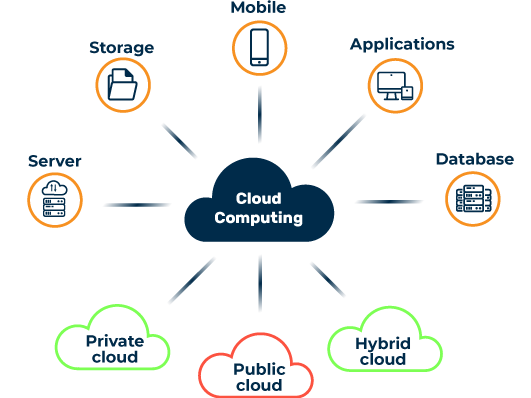
\includegraphics[scale=0.9]{sections/cloud-computing/images/cc.png}
    \caption{CC-Overview}
\end{figure}

Cloud Computing ist ein Modell, bei dem virtueller Speicher, jegliche Art von Server, Anwendungen nicht physisch, sondern rein über das Internet bereitgestellt werden. Diese werden in der Regel nach Bedarf als Teil eines As-a-Service-Modells angeboten. Mithilfe der Cloud werden Organisationsinterne Systeme und Rechenzentren mit virtuellen Ressourcen, wie Datenbanken und spezielle KI-und Rechensysteme ausgetauscht. Im Normalfall werden diese Ressourcen von externen Anbietern bereitgestellt und gewartet. 
\subsection{Vorteile von Cloud Computing}

Oft fallen, in Verbindung mit dem Thema Cloud Computing, Stichwörter wie „flexibel“ oder „agil“. Das liegt daran, dass gerade in heutigen Zeiten marktseitige und auch technologische Veränderungen schnell und oft vorgenommen werden. Deshalb betreiben viele Unternehmen sogenanntes Outsourcing, um nicht selbst für die Rechenleistung ihrer eigenen Dienste verantwortlich zu sein. Skalierbarkeit spielt hierbei eine große Rolle, ein Beispiel hierfür: je mehr Zugriffe auf einen Webshop erfolgen, desto mehr Ressourcen müssen im Hintergrund hochgefahren werden, um eine fehlerfrei Nutzung zu garantieren.

Auch die Usability ist simpler bei cloudbasierten Prozessen, da viele dieser Prozesse in den Hintergrund verschoben und somit von den Cloud Service-Anbietern übernommen werden. Der Aufwand für die  Wartung und Beschaffung für Rechenzentren entfällt weitgehend. Demzufolge kann man im Bereich Energie- und Erhaltungskosten einsparen. Im Allgemeinen werden die Kosten für ebensolche Dienste je nach Absprache nutzungsabhängig festgelegt. Im Normalfall fallen diese Kosten monatlich oder jährlich an, wobei diese verhältnismäßig kleiner als die der On-Premise Lösungen sind.

Ein essentieller Bestandteil ist die Datenkonsistenz. Im Fall von komplexen Prozessen ist die Konsistenz der Daten ein wesentlicher Punkt, um drastische Probleme zu verhindern. Gerade bei dezentraler Speicherung und Verarbeitung der Daten, ist die Synchronität überaus wichtig. Bei Cloud Computing ist dieses Risiko minimiert. Der Grund hierfür ist, dass die Daten, auch bei einem Zugriff von unterschiedlichen Schnittstellen synchron ist. 

\subsection{Hindernisse für den Einsatz einer Cloud}

Da es sich beim Cloud Computing um ein neues Modell handelt, besteht eine gewisse Unsicherheit, inwiefern es möglich ist, auf allen verschiedenen Ebenen eine solide Sicherheit zu erreichen. Dadurch wird die Fähigkeit der Cloud, den Datenschutzbestimmungen gerecht zu werden, in Frage gestellt. Das Grundprinzip der Cloud sieht eine dauerhafte Verfügbarkeit vor, jedoch kann gerade diese Verfügbarkeit auch ein großer Nachteil sein. Erst durch den offenen Zugang zu den zur Verfügungen gestellten Rechenleistung und anderen Ressourcen, entfaltet das CC-Model sein volles Potenzial. 

Heutzutage müssen Anwendungen dauerhaft erreichbar sein. Hierbei kann sich die Abhängigkeit von einem Cloud Service Provider negativ auf die dauerhafte Konnektivität auswirken. Im Fall von Aussetzern oder kompletten Ausfällen müssen Notfallpläne oder neue Ressourcen gestartet werden, um Datenverlust zu verhindern. 

